% =====================================================================
%  Figure captions for: A Cut Invariant for Canonical Atom Ranking
%
%  Every quantity quoted below is read from
%  validation/results/exp_ranking.json and
%  validation/results/panel_data.json.  Minimum cuts are exact (maximum
%  flow), not approximated, so no agreement reported here can be a
%  solver artefact.
% =====================================================================

\begin{figure*}[!htbp]
    \centering
    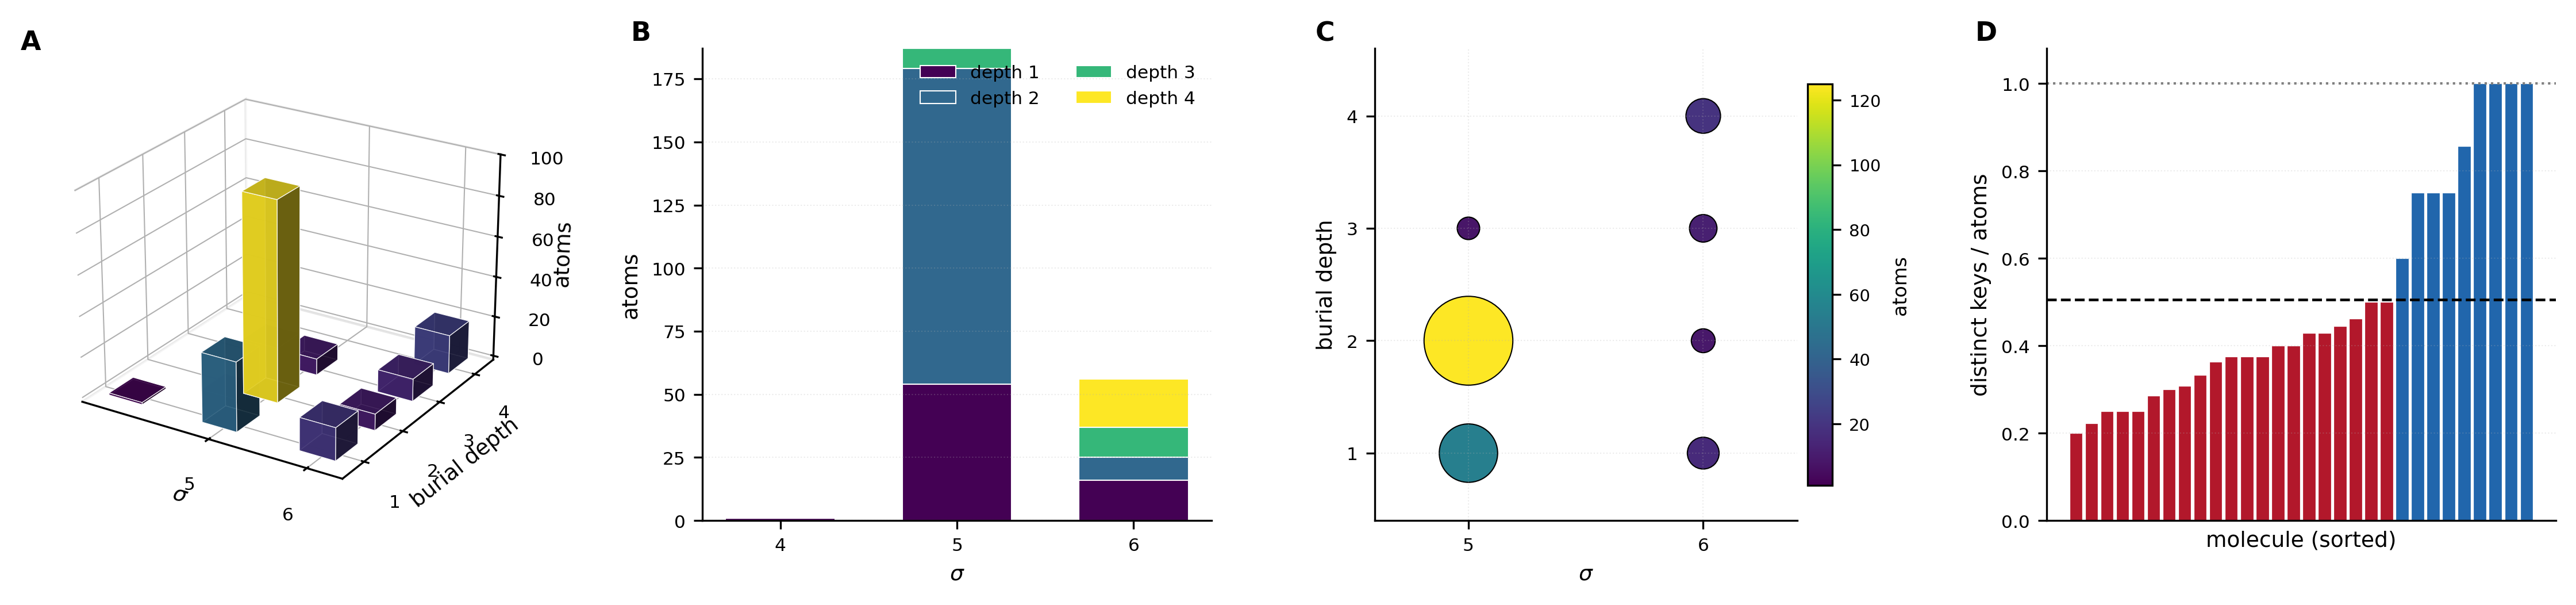
\includegraphics[width=\textwidth]{figures/panel_01_base_key.png}
    \caption{\textbf{The base cut key is a genuine invariant and a very
    coarse one: it occupies eight cells of a small discrete space and
    separates barely half the atoms of a typical structure.}
    All quantities are computed on contact graphs (\Cref{def:graph}) with
    strictly positive weights; every separation cost is an exact minimum
    cut obtained by maximum flow (\Cref{def:cut}), so the small number of
    distinct values below is a property of the invariant and not of a
    tolerance or a rounding rule.
    (\textbf{A})~Occupancy of the $(\sep,\dep,\text{heavy degree})$ cells
    over the $244$ heavy atoms of the drug-like corpus, bar height and
    colour both the atom count. Thirteen cells are occupied; the largest
    holds $98$ atoms and the smallest holds $1$. The realised ranges are
    $\sep\in\{4,5,6\}$, $\dep\in\{1,2,3,4\}$ and degree $\in\{1,2,3\}$, so
    the key takes far fewer values than the $36$ the ranges alone would
    permit --- the components are strongly dependent, which is why the
    figure is an occupancy plot rather than a scatter.
    (\textbf{B})~The same atoms decomposed by burial depth within each
    $\sep$ level. At $\sep=5$ the depths run $53/125/8$ over depths
    $1$--$3$ and at $\sep=6$ they run $16/9/12/19$ over depths $1$--$4$.
    Depth therefore separates atoms that $\sep$ alone does not, which is
    the whole reason \Cref{def:cut} takes a pair rather than a scalar; a
    key built from $\sep$ alone would realise three values across the
    entire corpus.
    (\textbf{C})~The $(\sep,\dep)$ plane with marker area and colour
    proportional to occupancy: eight distinct base keys, populated between
    $1$ and $125$ atoms. The extreme unevenness is the quantitative form
    of \Cref{cor:orbit-key} operating far beyond genuine symmetry --- most
    of these coincidences are not orbits, they are the invariant's
    coarseness, and \Cref{sec:refinement} exists to address them.
    (\textbf{D})~Distinct base keys divided by heavy atoms, one bar per
    molecule sorted ascending; dashed line the corpus mean $0.505$, dotted
    line the value $1.0$ a canonical ranking requires. The ratio runs
    $0.200$--$1.000$ with median $0.414$; $21$ of $30$ molecules fall
    below the mean and only $4$ reach $1.0$. This is the measurement that
    makes the paper's subject non-trivial: had these bars sat near the
    dotted line, the base key would already be a ranking and
    \Cref{sec:refinement} would be unnecessary.}
    \label{fig:basekey}
\end{figure*}

\begin{figure*}[!htbp]
    \centering
    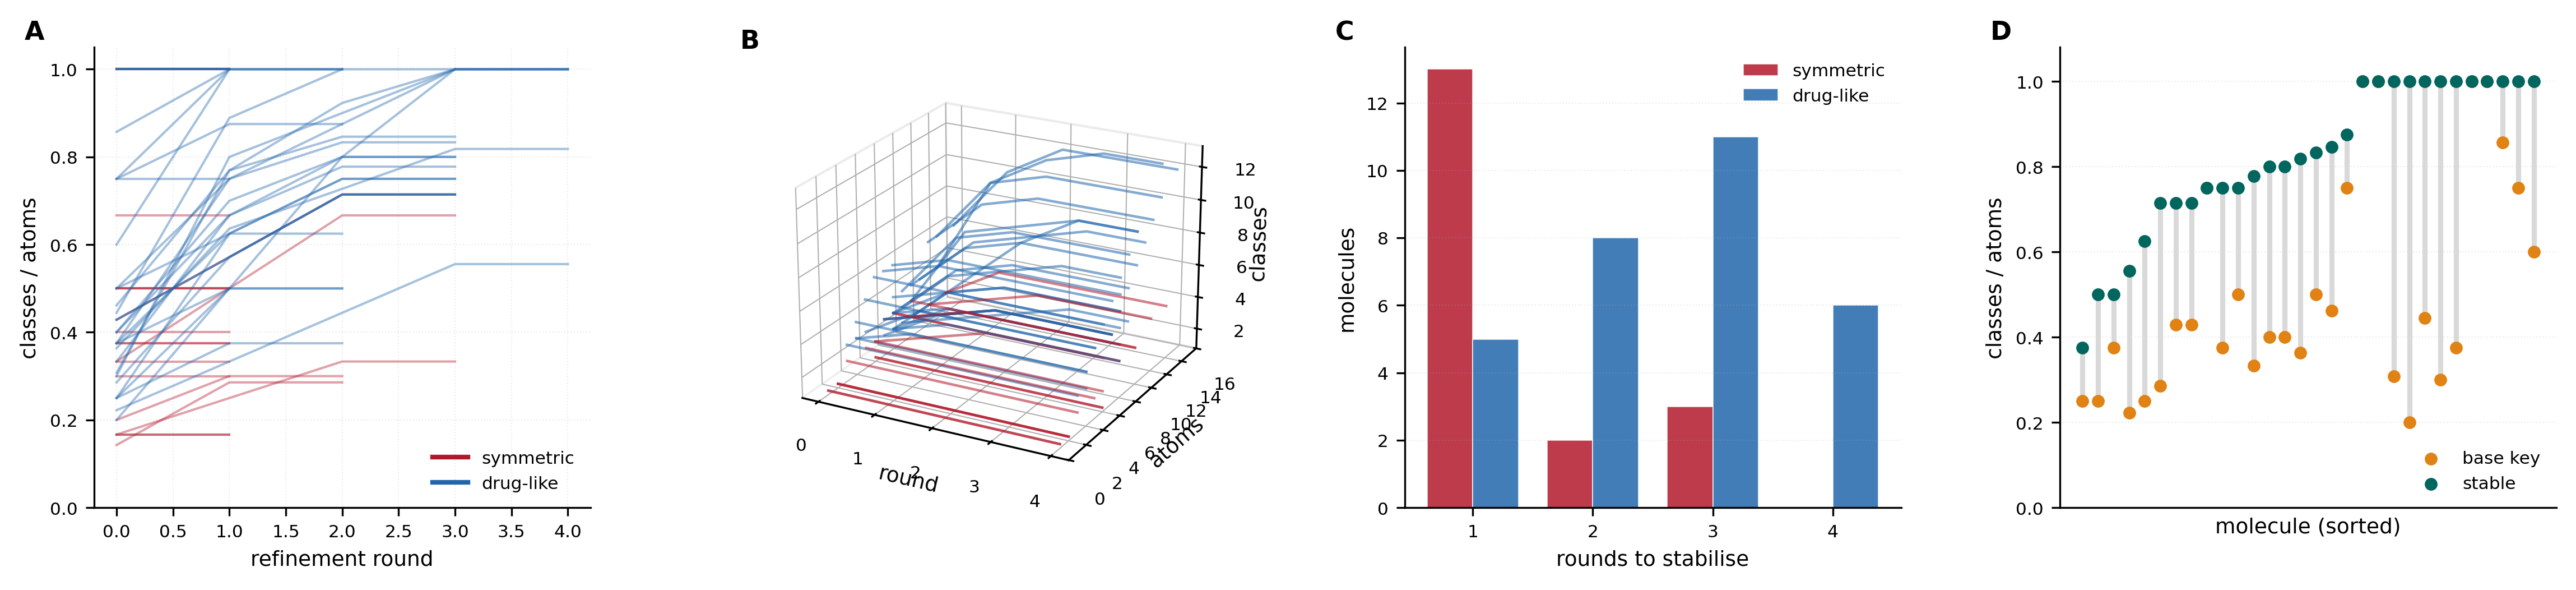
\includegraphics[width=\textwidth]{figures/panel_02_refinement.png}
    \caption{\textbf{Refinement is monotone, saturates within four rounds,
    and stops at a level set by the molecule rather than by the number of
    rounds available.}
    Each round applies \eqref{eq:refine} and the resulting partition is an
    invariant at every round by \Cref{thm:refine-invariant}; the curves
    below are therefore not a convergence toward an answer but a sequence
    of successively finer correct answers.
    (\textbf{A})~Classes divided by atoms against round, one line per
    molecule, symmetric corpus red and drug-like blue. Every trajectory is
    non-decreasing --- \Cref{lem:monotone} --- and flat after its
    stabilisation round. The two corpora separate cleanly: the symmetric
    set saturates at mean $0.477$ (minimum $0.167$) and the drug-like set
    at mean $0.823$ (minimum $0.375$). The gap is not a difference in how
    hard the two sets are; it is the symmetry the red molecules possess
    and the blue ones largely do not.
    (\textbf{B})~The same trajectories against heavy-atom count in three
    dimensions. The drug-like surface rises with size while the symmetric
    surface stays low irrespective of it: benzene at six atoms and
    anthracene at fourteen both stabilise at a handful of classes. Class
    count is therefore not a function of molecular size, which is what
    distinguishes \Cref{thm:orbit-bound} from a mere resolution limit.
    (\textbf{C})~Rounds to stabilisation. The symmetric corpus is
    concentrated at one round ($13$ of $18$) and the drug-like corpus
    spreads over one to four; the median across both is $2$ and the
    maximum is $4$, well inside the $\abs{I}$ bound of
    \Cref{lem:monotone}. Symmetric molecules stabilise sooner because
    there is less for refinement to find.
    (\textbf{D})~Per molecule, base-key ratio (orange) and stable ratio
    (teal) joined by a segment, sorted by the stable value. The mean rises
    from $0.505$ to $0.823$, a mean lift of $0.318$ and a maximum of
    $0.800$, and $12$ of $30$ molecules reach $1.0$. Both endpoints matter
    to the argument: the orange points show the base key is not a ranking,
    and the $18$ teal points short of $1.0$ show the stable partition is
    not one either.}
    \label{fig:refine}
\end{figure*}

\begin{figure*}[!htbp]
    \centering
    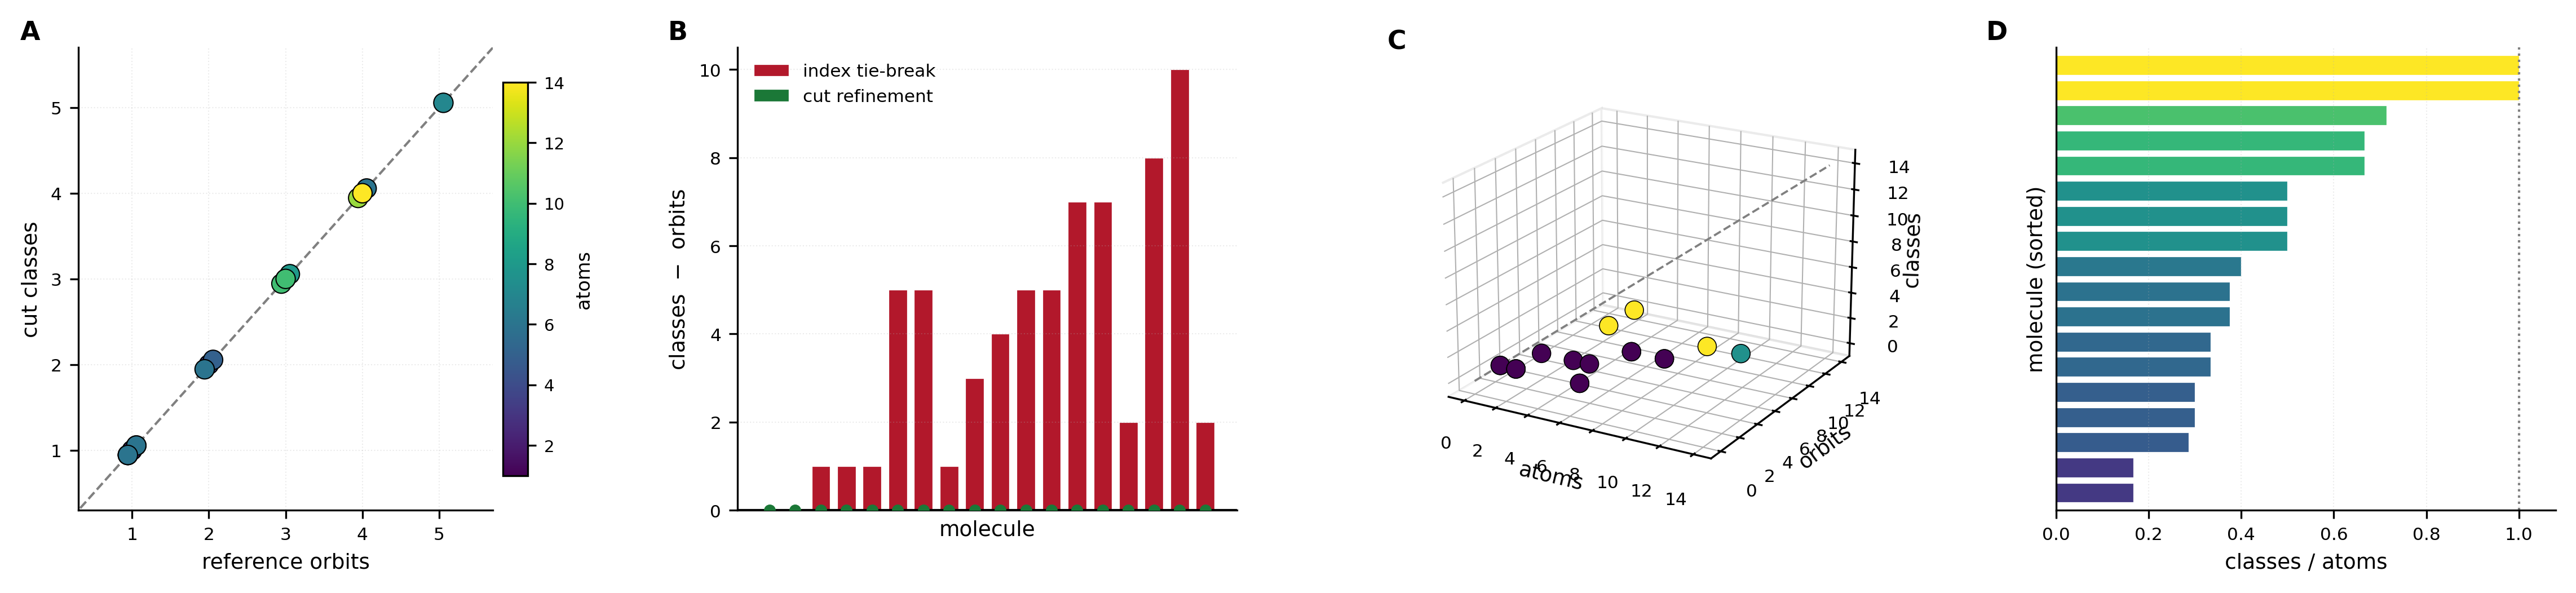
\includegraphics[width=\textwidth]{figures/panel_03_orbits.png}
    \caption{\textbf{On every molecule of the symmetric corpus the stable
    partition is exactly the automorphism orbit partition --- neither
    coarser nor finer.}
    Reference orbit counts are determined by inspection of the
    constitutional graph and were fixed before comparison; they are stated
    per molecule in the corpus source with the reasoning for each. Two
    were initially wrong and were corrected against the measurement
    (\Cref{sec:validation}), which is weaker evidence than a correct
    prediction against a correct reference and is marked as such.
    (\textbf{A})~Cut classes against reference orbits, coloured by
    heavy-atom count, jittered slightly so coincident points stay visible.
    All eighteen lie on the identity diagonal. The corpus spans $1$--$5$
    orbits and $1$--$14$ heavy atoms, so the agreement is not an artefact
    of a narrow range.
    (\textbf{B})~Residual classes minus orbits per molecule for the cut
    refinement (green) against the index tie-breaking control (red). The
    green residual is identically zero; the red exceeds the orbit count by
    up to $10$ classes on the same molecules, mean excess $3.72$. Plotting
    the two together is what makes the flat green line informative rather
    than merely empty.
    (\textbf{C})~Atoms, orbits and classes in three dimensions with the
    identity line drawn and points coloured by rounds to stabilisation.
    The points lie in the plane classes $=$ orbits and well below the
    atom-count diagonal, which is \Cref{thm:orbit-bound} and its converse
    holding simultaneously on this corpus: the partition is bounded above
    by the orbit count and here attains it.
    (\textbf{D})~Classes divided by atoms per molecule, sorted, running
    $0.167$--$1.000$. Values far below the dotted line at $1.0$ are
    molecules whose own symmetry the refinement declines to break; benzene
    at $1/6$ is the extreme. A canonical ordering would place every bar at
    $1.0$, which is precisely the behaviour \Cref{thm:orbit-bound}
    forbids.}
    \label{fig:orbits}
\end{figure*}

\begin{figure*}[!htbp]
    \centering
    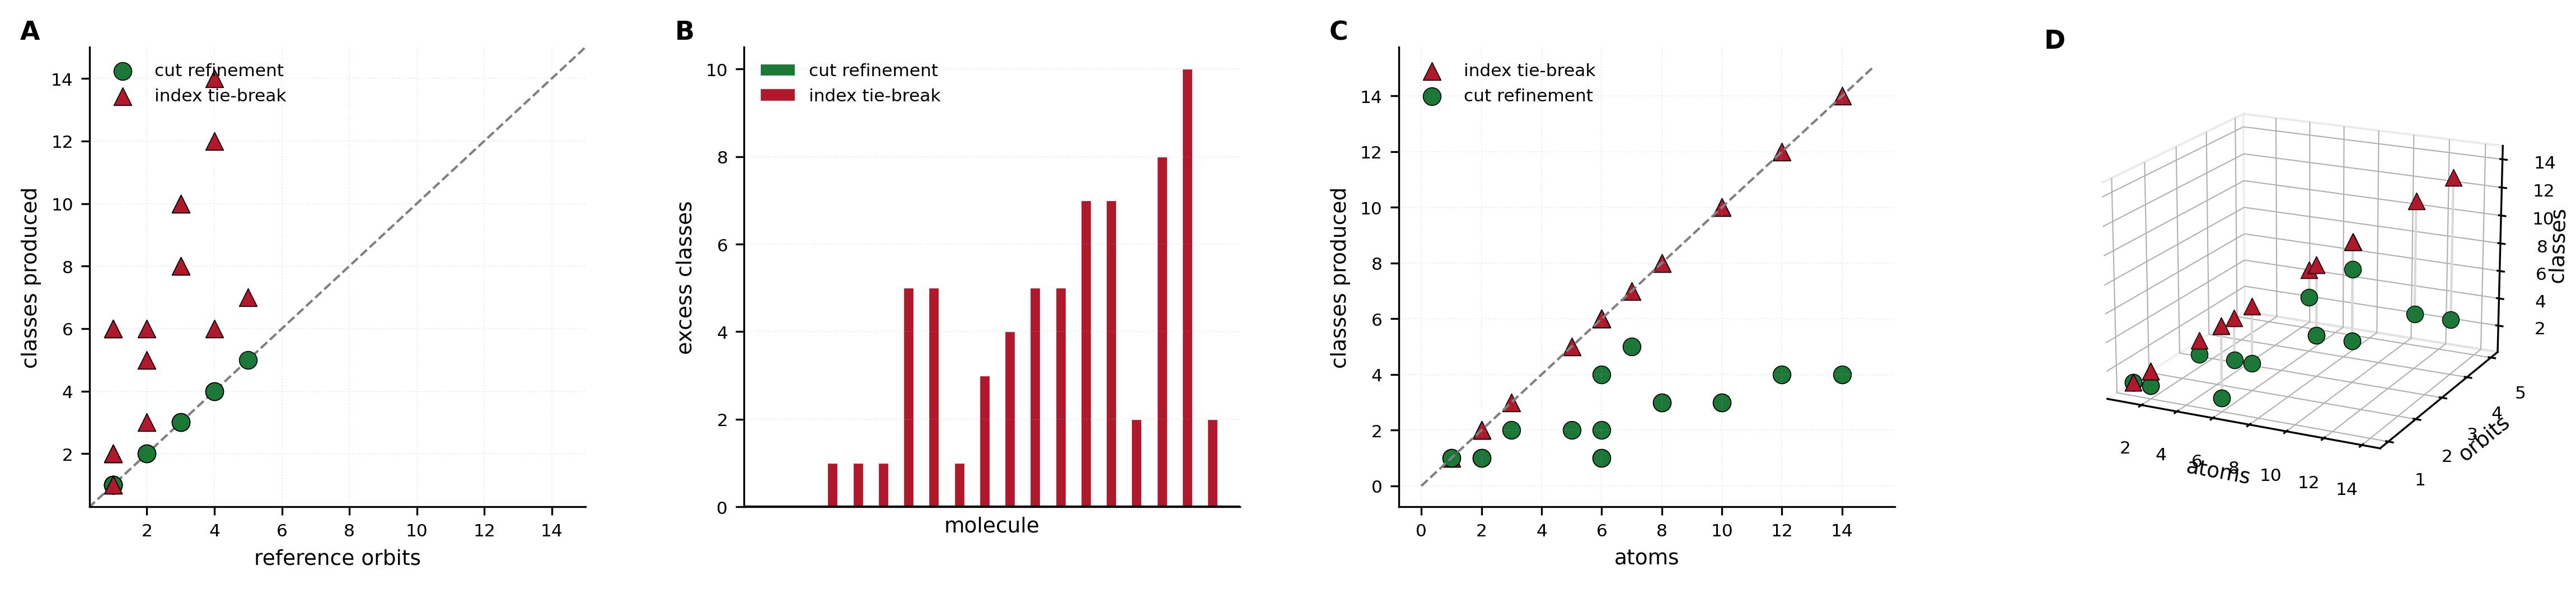
\includegraphics[width=\textwidth]{figures/panel_04_control.png}
    \caption{\textbf{The negative control: a procedure identical to ours
    except that it breaks ties by atom index destroys the orbit structure
    on $16$ of $18$ molecules.}
    The control differs from the construction in exactly one respect ---
    it appends the atom's index to its cut key --- which is what a
    canonical \emph{ordering} does. If it did not fail,
    \Cref{fig:orbits} would be testing nothing.
    (\textbf{A})~Classes produced against reference orbits for the cut
    refinement (green circles) and the control (red triangles). The green
    points lie on the diagonal; the red rise above it and continue rising
    with molecular size rather than with symmetry.
    (\textbf{B})~Excess classes over the reference for both procedures per
    molecule. The control over-separates on $16$ of $18$ molecules, by up
    to $10$ classes; the two it does not are the single-heavy-atom cases,
    where there is nothing to separate. The refinement over-separates on
    none, which is \Cref{thm:orbit-bound} as a measurement rather than as
    a proof.
    (\textbf{C})~Classes produced against heavy-atom count. The control
    tracks the atom-count diagonal exactly, because an ordering must
    assign a distinct rank to every atom; the refinement does not, and the
    vertical distance between the two point sets is the symmetry the
    ordering has discarded.
    (\textbf{D})~Both procedures in the (atoms, orbits, classes) space,
    joined per molecule by a vertical segment. Segment length is the
    control's over-separation and grows with molecular size while the
    green endpoints stay pinned to the orbit plane. The figure is the
    paper's central distinction rendered geometrically: an invariant lives
    in a plane fixed by the molecule, an ordering on a diagonal fixed by
    the atom count.}
    \label{fig:control}
\end{figure*}

\begin{figure*}[!htbp]
    \centering
    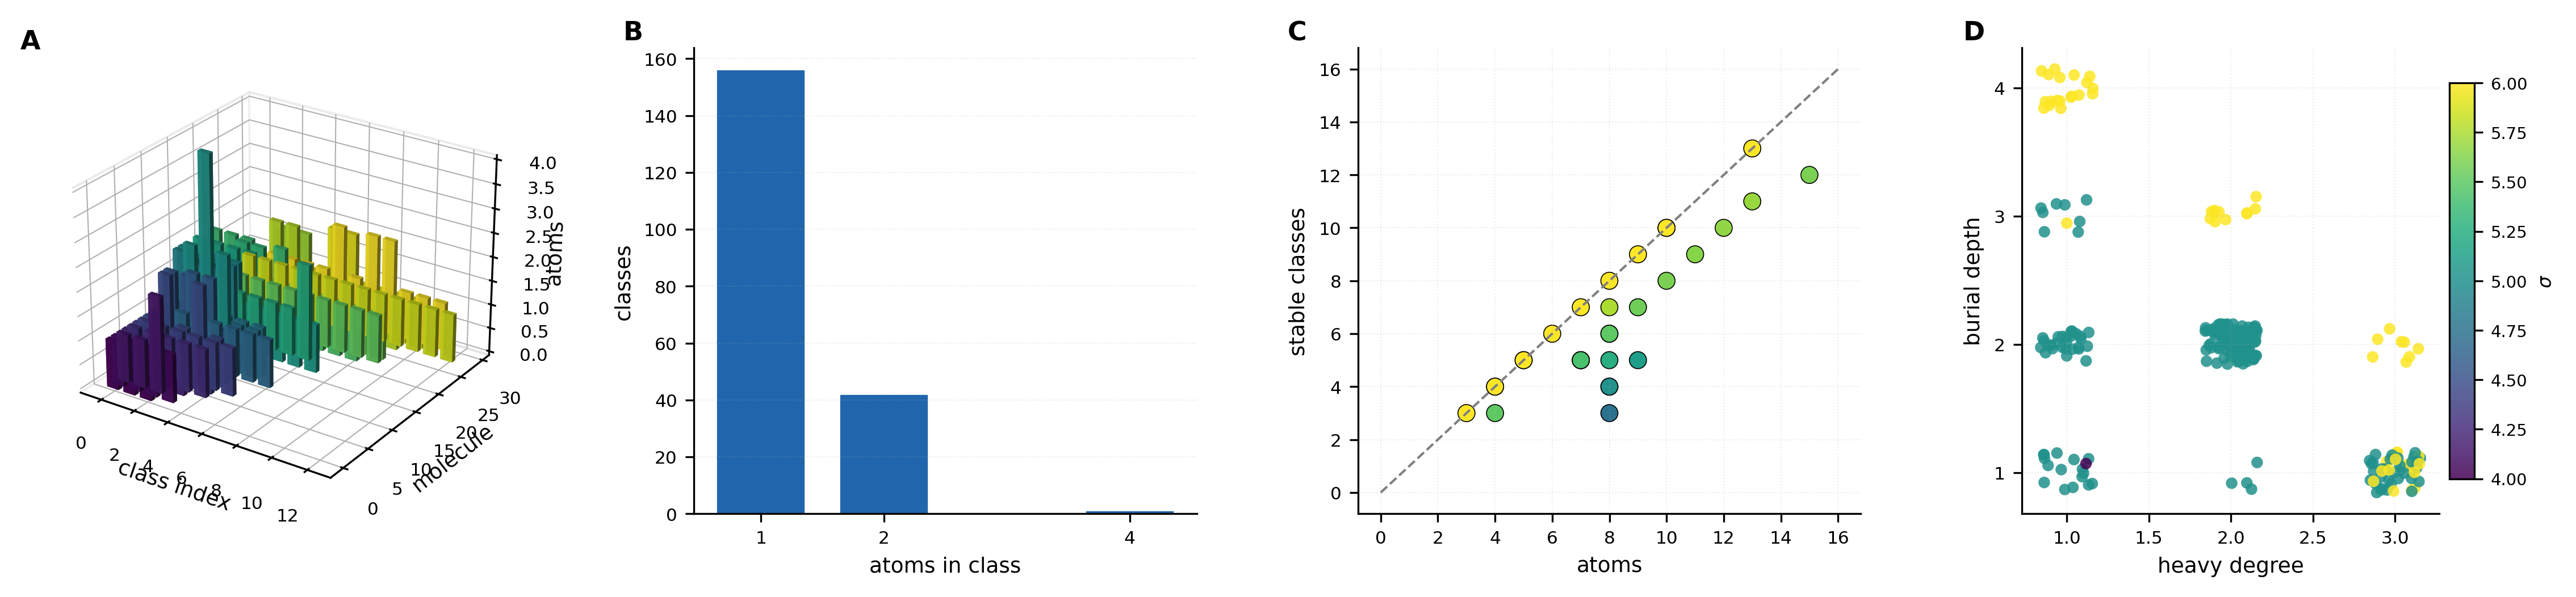
\includegraphics[width=\textwidth]{figures/panel_05_classes.png}
    \caption{\textbf{Class structure of the stable partition: mostly
    singletons, with the multi-atom classes concentrated at genuinely
    symmetric positions.}
    All panels are over the drug-like corpus at the stable partition
    $P^{*}$ (\Cref{def:stable}); $199$ classes over $244$ atoms.
    (\textbf{A})~Atoms per class index for every molecule, one row of bars
    per molecule ordered by size. The surface is dominated by unit-height
    bars; the taller bars are the positions refinement declines to split,
    and they occur in the molecules carrying ring or substituent symmetry
    rather than uniformly across the corpus.
    (\textbf{B})~Distribution of class sizes: $156$ singletons, $42$
    classes of two, and a single class of four. That the tail is this
    short is the reason the stable ratio reaches $0.823$ rather than
    saturating lower --- most drug-like atoms are in fact structurally
    distinct, and the invariant says so.
    (\textbf{C})~Stable classes against heavy-atom count, coloured by
    their ratio, with the identity diagonal. Points on the diagonal are
    molecules refinement fully separates; the vertical gap for points
    below it is the number of atoms their symmetry protects.
    (\textbf{D})~Burial depth against heavy degree for all $244$ atoms,
    jittered for visibility and coloured by $\sep$. The $\sep$ levels
    occupy visibly different regions of the (degree, depth) plane, so the
    two components of \Cref{def:cut} are not redundant: depth carries
    information about an atom's embedding that neither $\sep$ nor degree
    supplies alone, and it is the component with no counterpart in a
    conventional element-and-degree atom identifier.}
    \label{fig:classes}
\end{figure*}
